\section{Tutorial A10.4}

\begin{problem}
    A complex number $z$ is represented in an Argand diagram by the point $P$. Sketch, on separate Argand diagrams, the locus of $P$. Describe geometrically the locus of $P$ and determine its Cartesian equation.

    \begin{enumerate}
        \item $\abs{2z - 6 - 8\i} = 10$
        \item $\abs{z + 2} = \abs{z - \i}$
        \item $\arg{z + 2 - \i} = -\pi/4$
    \end{enumerate}
\end{problem}
\begin{solution}
    \begin{ppart}
        Note that $\abs{2z - 6 - 8\i} = 10 \implies \abs{z - (3 + 4\i)} = 5$.

        \begin{center}\tikzsetnextfilename{79}
            \begin{tikzpicture}[trim axis left, trim axis right]
                \begin{axis}[
                    domain = 0:10,
                    samples = 101,
                    axis y line=middle,
                    axis x line=middle,
                    xtick = \empty,
                    ytick = \empty,
                    xmax=11.5,
                    xmin=-5.5,
                    ymin=-4,
                    ymax=11,
                    xlabel = {$\Re$},
                    ylabel = {$\Im$},
                    legend cell align={left},
                    legend pos=outer north east,
                    after end axis/.code={
                        \path (axis cs:0,0) 
                            node [anchor=north east] {$O$};
                        }
                    ]
        
                    \coordinate (O) at (0, 0);
                    \coordinate[label=right:$3 + 4\i$] (C) at (3, 4);

                    \fill (C) circle[radius=2.5pt];

                    \draw[<->] (O) -- (C);

                    \node[anchor=west] at (1.7, 2) {$5$};

                    \draw[plotRed] (C) circle[radius=5];
                    
                    \addlegendimage{no markers, plotRed}
                    \addlegendentry{locus of $P$};
                \end{axis}
            \end{tikzpicture}
        \end{center}

        The locus of $P$ is a circle with centre $(3, 4)$ and radius $5$. Its Cartesian equation is $(x-3)^2 + (y-4)^2 = 5^2$.
    \end{ppart}
    \begin{ppart}
        Note that $\abs{z + 2} = \abs{z - \i} \implies \abs{z - (-2)} = \abs{z - \i}$.

        \begin{center}\tikzsetnextfilename{80}
            \begin{tikzpicture}[trim axis left, trim axis right]
                \begin{axis}[
                    domain = -10:10,
                    samples = 101,
                    axis y line=middle,
                    axis x line=middle,
                    xtick = {-2},
                    ytick = {1},
                    yticklabels = {$\i$},
                    xmax=2,
                    xmin=-3,
                    ymin=-2,
                    ymax=2,
                    xlabel = {$\Re$},
                    ylabel = {$\Im$},
                    legend cell align={left},
                    legend pos=outer north east,
                    after end axis/.code={
                        \path (axis cs:0,0) 
                            node [anchor=north west] {$O$};
                        }
                    ]
        
                    \coordinate (Z1) at (-2, 0);
                    \coordinate (Z2) at (0, 1);
                    \coordinate (O) at (0, 0);

                    \draw[dotted] (Z1) -- (Z2);

                    \addplot[plotRed] {-2*x - 1.5};
            
                    \fill (Z1) circle[radius=2.5pt];
                    \fill (Z2) circle[radius=2.5pt];

                    \addlegendentry{locus of $P$};

                    \coordinate (Z3) at (0, -1.5);
                    \coordinate (Z4) at (-1, 0.5);
                    \draw pic [draw, angle radius=3mm, ""] {right angle =  Z3--Z4--Z2};

                    \draw ($(-1.5, 0.25)!0.2cm!270:(Z1)$) -- ($(-1.5, 0.25)!0.2cm!90:(Z1)$);
                    \draw ($(-0.5, 0.75)!0.2cm!270:(Z1)$) -- ($(-0.5, 0.75)!0.2cm!90:(Z1)$);
                \end{axis}
            \end{tikzpicture}
        \end{center}

        The locus of $P$ is the perpendicular bisector of the line segment joining $(-2, 0)$ and $(0, 1)$. Its Cartesian equation is $y = -2x - 1.5$.
    \end{ppart}
    \begin{ppart}
        Note that $\arg{z + 2 - \i} = -\pi/4 \implies \arg{z - (-2 + \i)} = -\pi/4$.

        \begin{center}\tikzsetnextfilename{81}
            \begin{tikzpicture}[trim axis left, trim axis right]
                \begin{axis}[
                    domain = -2:3,
                    samples = 101,
                    axis y line=middle,
                    axis x line=middle,
                    xtick = {-2},
                    ytick = {1},
                    yticklabels = {$\i$},
                    xmax=2,
                    xmin=-3,
                    ymin=-2,
                    ymax=2,
                    xlabel = {$\Re$},
                    ylabel = {$\Im$},
                    legend cell align={left},
                    legend pos=outer north east,
                    after end axis/.code={
                        \path (axis cs:0,0) 
                            node [anchor=north west] {$O$};
                        }
                    ]
        
                    \coordinate[label=above:$-2+\i$] (Z1) at (-2, 1);
                    \coordinate (Z2) at (0, 1);
                    \coordinate (O) at (0, 0);

                    \draw[dotted] (Z1) -- (Z2);

                    \addplot[plotRed] {-x - 1};
            
                    \draw (Z1) circle[radius=2.5pt];

                    \addlegendentry{locus of $P$};

                    \coordinate (Z3) at (0, -1);
                    \draw pic [draw, angle radius=12mm, "$-\frac\pi4$"] {angle =  Z3--Z1--Z2};
                \end{axis}
            \end{tikzpicture}
        \end{center}
            
        The locus of $P$ is the half-line starting from $(-2, 1)$ and inclined at an angle $-\pi/4$ to the positive real axis. Its Cartesian equation is $y = -x - 1$
    \end{ppart}
\end{solution}

\begin{problem}
    Sketch the following loci on separate Argand diagrams.

    \begin{enumerate}
        \item $\Re{z^2} = 1$
        \item $\abs{6 - \i z} = 2$,
        \item $\arg{\frac{\i z}{1 - \sqrt3 \i}} = \pi$
    \end{enumerate}
\end{problem}
\begin{solution}
    \begin{ppart}
        Let $z = r(\cos \t + \i\sin \t)$. Then $\Re{z^2} = 1 \implies r^2 \cos 2\t = 1 \implies r^2 = \sec 2\t$.

        \begin{center}\tikzsetnextfilename{82}
            \begin{tikzpicture}[trim axis left, trim axis right]
                \begin{axis}[
                    domain = 0:2*pi,
                    samples = 100,
                    axis y line=middle,
                    axis x line=middle,
                    xtick = {-1, 1},
                    ytick = \empty,
                    xmin=-2,
                    xmax=2,
                    ymin=-2,
                    ymax=2,
                    xlabel = {$\Re$},
                    ylabel = {$\Im$},
                    legend cell align={left},
                    legend pos=outer north east,
                    after end axis/.code={
                        \path (axis cs:0,0) 
                            node [anchor=north east] {$O$};
                        }
                    ]
                    \addplot[color=plotRed,data cs=polarrad] {1/sqrt(cos(2 * \x r))};
        
                    \addlegendentry{required locus};
                \end{axis}
            \end{tikzpicture}
        \end{center}
    \end{ppart}
    \begin{ppart}
        Note $\abs{6 - \i z} = 2 \implies \abs{-\i (z + 6i)} = 2 \implies \abs{z + 6\i} = 2 \implies \abs{z - (6\i)} = 2$.

        \begin{center}\tikzsetnextfilename{83}
            \begin{tikzpicture}[trim axis left, trim axis right]
                \begin{axis}[
                    domain = 0:10,
                    samples = 101,
                    axis y line=middle,
                    axis x line=middle,
                    xtick = \empty,
                    ytick = {-6},
                    yticklabels = {$-6\i$},
                    xmax=6,
                    xmin=-6,
                    ymin=-9,
                    ymax=1,
                    xlabel = {$\Re$},
                    ylabel = {$\Im$},
                    legend cell align={left},
                    legend pos=outer north east,
                    after end axis/.code={
                        \path (axis cs:0,0) 
                            node [anchor=north east] {$O$};
                        }
                    ]
        
                    \coordinate (O) at (0, 0);
                    \coordinate (C) at (0, -6);

                    \fill (C) circle[radius=2.5pt];

                    \draw[<->] (2, -6) -- (C);

                    \node[anchor=south] at (1, -6) {$2$};

                    \draw[plotRed] (C) circle[radius=2];
                    
                    \addlegendimage{no markers, plotRed}
                    \addlegendentry{required locus};
                \end{axis}
            \end{tikzpicture}
        \end{center}
    \end{ppart}
    \begin{ppart}
        Note $\arg{\frac{\i z}{1 - \sqrt3 \i}} = \pi \implies \frac\pi2 + \arg{z} - \bp{-\frac\pi3} \implies \arg{z} = \frac\pi6$.

        \begin{center}\tikzsetnextfilename{84}
            \begin{tikzpicture}[trim axis left, trim axis right]
                \begin{axis}[
                    domain = 0:3 ,
                    samples = 101,
                    axis y line=middle,
                    axis x line=middle,
                    xtick = \empty,
                    ytick = \empty,
                    xmax=3,
                    xmin=-0.5,
                    ymin=-0.5,
                    ymax=2,
                    xlabel = {$\Re$},
                    ylabel = {$\Im$},
                    legend cell align={left},
                    legend pos=outer north east,
                    after end axis/.code={
                        \path (axis cs:0,0) 
                            node [anchor=north west] {$O$};
                        }
                    ]
        
                    \coordinate (Z1) at (0.866, 0.5);
                    \coordinate (O) at (0, 0);

                    \addplot[plotRed] {0.5774 * x};
            
                    \draw (O) circle[radius=2.5pt];

                    \addlegendentry{required locus};

                    \coordinate (Z2) at (1, 0);
                    \draw pic [draw, angle radius=14mm, "$-\frac\pi4$"] {angle =  Z2--O--Z1};
                \end{axis}
            \end{tikzpicture}
        \end{center}
    \end{ppart}
\end{solution}

\begin{problem}
    Sketch, on separate Argand diagrams, the set of points satisfying the following inequalities.

    \begin{enumerate}
        \item $2 < \abs{z - 2\i} \leq \abs{3 - 4\i}$
        \item $\abs{z + \i} > \abs{z + 1 - \i}$
        \item $\frac\pi4 < \arg{\frac1z} \leq \frac\pi2$
    \end{enumerate}
\end{problem}
\begin{solution}
    \begin{ppart}
        Note $2 < \abs{z - 2\i} \leq \abs{3 - 4\i} \implies 2 < \abs{z - 2\i} \leq 5$.

        \begin{center}\tikzsetnextfilename{85}
            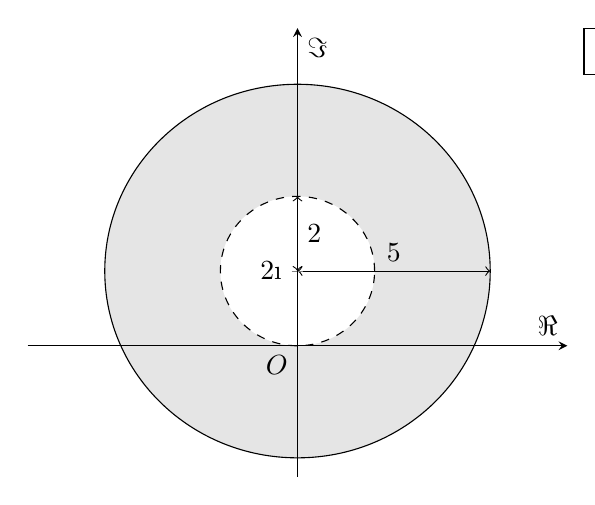
\begin{tikzpicture}[trim axis left, trim axis right]
                \pgfdeclarelayer{pre main}
                \pgfsetlayers{pre main,main}
                \begin{axis}[
                    axis on top,
                    domain = 0:3 ,
                    samples = 101,
                    axis y line=middle,
                    axis x line=middle,
                    xtick = \empty,
                    ytick = {2},
                    yticklabels = {$2\i$},
                    ymax=8.5,
                    ymin=-3.5,
                    xmin=-7,
                    xmax=7,
                    xlabel = {$\Re$},
                    ylabel = {$\Im$},
                    legend cell align={left},
                    legend pos=outer north east,
                    after end axis/.code={
                        \path (axis cs:0,0) 
                            node [anchor=north east] {$O$};
                        }
                    ]
                    \coordinate (Z1) at (0, 2);
                    \pgfonlayer{pre main}
                    \fill[black!10] (Z1) circle[radius=5];
                    \endpgfonlayer
                    \fill[white] (Z1) circle[radius=2];

                    \coordinate (O) at (0, 0);

                    \draw (Z1) circle[radius=5];
                    \draw[dashed] (Z1) circle[radius=2];

                    \addlegendimage{line legend, black!10, line width=5pt}
                    \addlegendentry{required locus};

                    \draw[<->] (Z1) -- (5, 2);
                    \draw[<->] (Z1) -- (0, 4);

                    \node[anchor=south] at (2.5, 2) {$5$};
                    \node[anchor=west] at (0, 3) {$2$};
                \end{axis}
            \end{tikzpicture}
        \end{center}
    \end{ppart}
    \begin{ppart}
        Note $\abs{z + \i} > \abs{z + 1 - \i} \implies \abs{z - (-\i)} > \abs{z - (-1 + \i)}$.

        \begin{center}\tikzsetnextfilename{86}
            \begin{tikzpicture}[trim axis left, trim axis right]
                \pgfdeclarelayer{pre main}
                \pgfsetlayers{pre main,main}
                \begin{axis}[
                    axis on top,
                    domain = -4:10 ,
                    samples = 101,
                    axis y line=middle,
                    axis x line=middle,
                    xtick = \empty,
                    ytick = {-1},
                    yticklabels = {$-\i$},
                    ymax=4,
                    ymin=-2,
                    xmin=-4.5,
                    xmax=2.5,
                    xlabel = {$\Re$},
                    ylabel = {$\Im$},
                    legend cell align={left},
                    legend pos=outer north east,
                    after end axis/.code={
                        \path (axis cs:0,0) 
                            node [anchor=north west] {$O$};
                        }
                    ]
                    \pgfonlayer{pre main}
                    \fill[black!10] (-4, -1.75) rectangle (2.5, 4);
                    \endpgfonlayer
                
                    \coordinate[label=above left:$-1+\i$] (Z1) at (-1, 1);
                    \coordinate (Z2) at (0, -1);

                    \addlegendimage{line legend, black!10, line width=5pt}
                    \addlegendentry{required locus};

                    \fill (Z1) circle[radius=2.5pt];
                    \fill (Z2) circle[radius=2.5pt];

                    \draw[dotted] (Z1) -- (Z2);
                    \addplot[dashed, black, name path=f1] {0.5 * x + 0.25};

                    \addplot[thin, name path=null, white] {-1.75};
                    \addplot[color=white] fill between[of=null and f1,soft clip={domain=-4:5}];

                    \coordinate (Z3) at (-0.5, 0);
                    \coordinate (Z4) at (0, 0.25);

                    \draw pic [draw, angle radius=3mm, ""] {right angle = Z4--Z3--Z1};

                    \draw ($(-0.75, 0.5)!0.2cm!270:(Z1)$) -- ($(-0.75, 0.5)!0.2cm!90:(Z1)$);
                    \draw ($(-0.25, -0.5)!0.2cm!270:(Z1)$) -- ($(-0.25, -0.5)!0.2cm!90:(Z1)$);
                \end{axis}
            \end{tikzpicture}
        \end{center}
    \end{ppart}
    \begin{ppart}
        Note $\frac\pi4 < \arg{\frac1z} \leq \frac\pi2 \implies \frac\pi4 < -\arg{z} \leq \frac\pi2 \implies -\frac\pi2 \geq \arg{z} > -\frac\pi4$.

        \begin{center}\tikzsetnextfilename{87}
            \begin{tikzpicture}[trim axis left, trim axis right]
                \pgfdeclarelayer{pre main}
                \pgfsetlayers{pre main,main}
                \begin{axis}[
                    axis on top,
                    domain = -4:10 ,
                    samples = 101,
                    axis y line=middle,
                    axis x line=middle,
                    xtick = \empty,
                    ytick = \empty,
                    ymax=1,
                    ymin=-5,
                    xmin=-1,
                    xmax=7,
                    xlabel = {$\Re$},
                    ylabel = {$\Im$},
                    legend cell align={left},
                    legend pos=outer north east,
                    after end axis/.code={
                        \path (axis cs:0,0) 
                            node [anchor=north east] {$O$};
                        }
                    ]
                    \pgfonlayer{pre main}
                    \fill[black!10] (0, 0) rectangle (5, -5);
                    \endpgfonlayer

                    \addlegendimage{line legend, black!10, line width=5pt}
                    \addlegendentry{required locus};

                    \coordinate (O) at (0, 0);
                    \coordinate (Z1) at (5, -5);
                    \draw (O) circle[radius=2.5pt];

                    \addplot[dashed, domain=0:5, name path=f1] {-x};
                    
                    \addplot[thin, name path=null, white] {0};
                    \addplot[color=white] fill between[of=null and f1,soft clip={domain=0:5}];

                    \coordinate (Z2) at (5, 0);
                    \draw pic [draw, angle radius=12mm, "$-\frac\pi4$"] {angle = Z1--O--Z2};
                \end{axis}
            \end{tikzpicture}
        \end{center}
    \end{ppart}
\end{solution}

\begin{problem}
    Sketch on separate Argand diagrams for (a) and (b) the set of points representing all complex numbers $z$ satisfying both of the following inequalities.

    \begin{enumerate}
        \item $\abs{z - 3 - \i} \leq 3$ and $\abs{z} \geq \abs{z - 3 - \i}$
        \item $\frac\pi2 < \arg{z + 1} \leq \frac23 \pi$ and $3 \Im{z} > 2$
    \end{enumerate}
\end{problem}
\begin{solution}
    \begin{ppart}
        Note $\abs{z - 3 - \i} \leq 3 \implies \abs{z - (3 + \i)} \leq 3$ and $\abs{z} \geq \abs{z - 3 - \i} \implies \abs{z} \geq \abs{z - (3 + \i)}$.

        \begin{center}\tikzsetnextfilename{88}
            \begin{tikzpicture}[trim axis left, trim axis right]
                \pgfdeclarelayer{pre main}
                \pgfsetlayers{pre main,main}
                \begin{axis}[
                    axis on top,
                    domain = -4:10 ,
                    samples = 101,
                    axis y line=middle,
                    axis x line=middle,
                    xtick = \empty,
                    ytick = \empty,
                    ymax=5,
                    ymin=-3,
                    xmin=-2,
                    xmax=7.5,
                    xlabel = {$\Re$},
                    ylabel = {$\Im$},
                    legend cell align={left},
                    legend pos=outer north east,
                    after end axis/.code={
                        \path (axis cs:0,0) 
                            node [anchor=north east] {$O$};
                        }
                    ]
                    \addlegendimage{line legend, black!10, line width=5pt}
                    \addlegendentry{required locus};

                    \coordinate (O) at (0, 0);
                    \coordinate[label=above:$3 + \i$] (Z) at (3, 1);

                    \fill (O) circle[radius=2.5pt];
                    \fill (Z) circle[radius=2.5pt];
                    \draw (Z) circle[radius=3];

                    \draw[dotted] (O) -- (Z);

                    \pgfonlayer{pre main}
                        \fill[black!10] (Z) circle[radius=3];
                    \endpgfonlayer

                    
                    \addplot[black, name path=f1] {5 - 3*x};
                    \addplot[thin, name path=null, white] {-2.5};
                    \addplot[color=white] fill between[of=null and f1,soft clip={domain=0:6}];

                    \coordinate (Z1) at (0, 5);
                    \coordinate (Z2) at (1.5, 0.5);

                    \draw pic [draw, angle radius=3mm, ""] {right angle = Z1--Z2--O};

                    \draw[<->] (Z) -- (3, -2);
                    \node[anchor=west] at (3, -1) {$3$};
                \end{axis}
            \end{tikzpicture}
        \end{center}
    \end{ppart}
    \begin{ppart}
        Note $\frac\pi2 < \arg{z + 1} < \frac23 \pi \implies \frac\pi2 < \arg{z - (-1)} < \frac23 \pi$ and $3\Im{z} > 2 \implies \Im{z} > \frac23$.

        \begin{center}\tikzsetnextfilename{89}
            \begin{tikzpicture}[trim axis left, trim axis right]
                \pgfdeclarelayer{pre main}
                \pgfsetlayers{pre main,main}
                \begin{axis}[
                    axis on top,
                    domain = -4:10 ,
                    samples = 101,
                    axis y line=middle,
                    axis x line=middle,
                    xtick = {-1},
                    ytick = {2/3},
                    yticklabels = {$\frac23 \i$},
                    ymax=3,
                    ymin=-1,
                    xmin=-3,
                    xmax=1,
                    xlabel = {$\Re$},
                    ylabel = {$\Im$},
                    legend cell align={left},
                    legend pos=outer north east,
                    after end axis/.code={
                        \path (axis cs:0,0) 
                            node [anchor=north east] {$O$};
                        }
                    ]
                    \addlegendimage{line legend, black!10, line width=5pt}
                    \addlegendentry{required locus};

                    \coordinate (O) at (0, 0);
                    \coordinate (Z) at (-1, 0);

                    \fill (Z) circle[radius=2.5pt];

                    \pgfonlayer{pre main}
                        \fill[black!10] (-2, 2/3-0.01) rectangle (-1, 3);
                    \endpgfonlayer
                    
                    \addplot[black, name path=f1, domain=-3:-1, dashed] {-3*(x + 1)};
                    \addplot[thin, name path=null, white] {2/3};
                    \addplot[color=white] fill between[of=null and f1,soft clip={domain=-3:-1}];

                    \addplot[dashed] {2/3};

                    \draw[dashed] (Z) -- (-1, 5);
                \end{axis}
            \end{tikzpicture}
        \end{center}
    \end{ppart}
\end{solution}

\begin{problem}
    Illustrate, in separate Argand diagrams, the set of points $z$ for which
        
    \begin{enumerate}
        \item $\Re{z^2} < 0$
        \item $\Im{z^3} > 0$
    \end{enumerate}
\end{problem}
\begin{solution}
    \begin{ppart}
        Let $z = r(\cos \t + \i\sin\t)$, $0 \leq \t < 2\pi$. Then $\Re(z^2) < 0 \implies r^2\cos 2\t < 0 \implies \cos 2\t < 0 \implies 2\t \in \bp{\frac12\pi, \frac32\pi} \cup \bp{\frac52 \pi, \frac72 \pi} \implies \t \in \bp{\frac14\pi, \frac34 \pi} \cup \bp{\frac54 \pi, \frac74 \pi}$.

        \begin{center}\tikzsetnextfilename{90}
            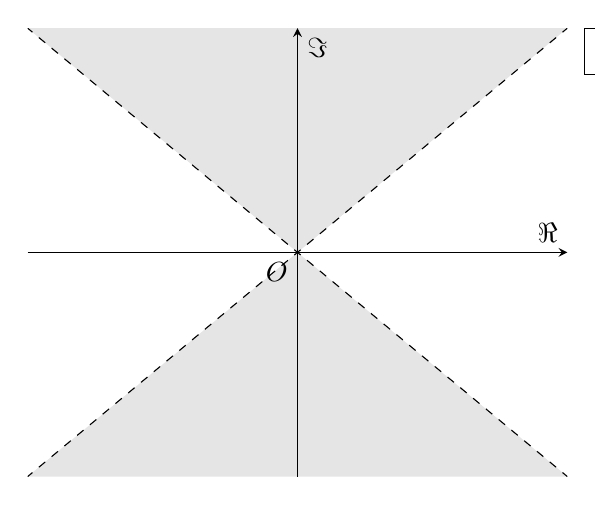
\begin{tikzpicture}[trim axis left, trim axis right]
                \pgfdeclarelayer{pre main}
                \pgfsetlayers{pre main,main}
                \begin{axis}[
                    axis on top,
                    domain = -10:10 ,
                    samples = 101,
                    axis y line=middle,
                    axis x line=middle,
                    xtick = \empty,
                    ytick = \empty,
                    xmax=5,
                    xmin=-5,
                    ymin=-5,
                    ymax=5,
                    xlabel = {$\Re$},
                    ylabel = {$\Im$},
                    legend cell align={left},
                    legend pos=outer north east,
                    after end axis/.code={
                        \path (axis cs:0,0) 
                            node [anchor=north east] {$O$};
                        }
                    ]
                    \addlegendimage{line legend, black!10, line width=5pt}
                    \addlegendentry{required locus};
                    
                    \addplot[dashed] {x};
                    \addplot[dashed] {-x};

                    \pgfonlayer{pre main}
                        \fill[black!10] (-5, 5) -- (0, 0) -- (5, 5) -- cycle;
                        \fill[black!10] (-5, -5) -- (0, 0) -- (5, -5) -- cycle;
                    \endpgfonlayer
                \end{axis}
            \end{tikzpicture}
        \end{center}
    \end{ppart}
    \clearpage
    \begin{ppart}
        Let $z = r(\cos \t + \i\sin\t)$, $0 \leq \t < 2\pi$. Then $\Im(z^3) > 0 \implies r^3\sin 3\t > 0 \implies \sin 3\t > 0 \implies 3\t \in \bp{0, \pi} \cup \bp{2\pi, 3\pi} \cup \bp{4\pi, 5\pi} \implies \t \in \bp{0, \frac13 \pi} \cup \bp{\frac23 \pi, \pi} \cup \bp{\frac43\pi, \frac53 \pi}$.

        \begin{center}\tikzsetnextfilename{91}
            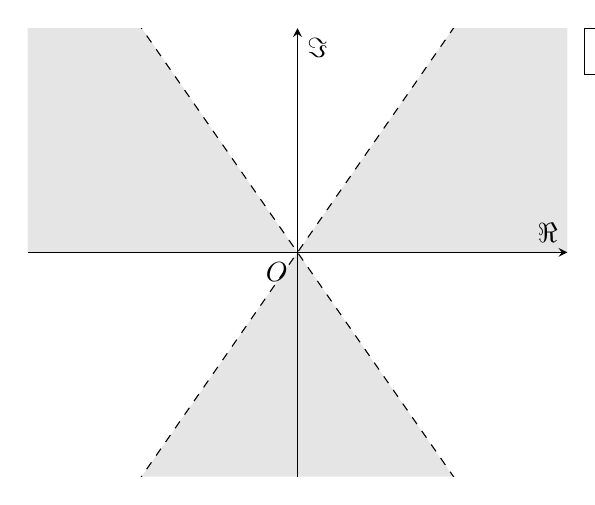
\begin{tikzpicture}[trim axis left, trim axis right]
                \pgfdeclarelayer{pre main}
                \pgfsetlayers{pre main,main}
                \begin{axis}[
                    axis on top,
                    domain = -10:10 ,
                    samples = 101,
                    axis y line=middle,
                    axis x line=middle,
                    xtick = \empty,
                    ytick = \empty,
                    xmax=5,
                    xmin=-5,
                    ymin=-5,
                    ymax=5,
                    xlabel = {$\Re$},
                    ylabel = {$\Im$},
                    legend cell align={left},
                    legend pos=outer north east,
                    after end axis/.code={
                        \path (axis cs:0,0) 
                            node [anchor=north east] {$O$};
                        }
                    ]
                    \addlegendimage{line legend, black!10, line width=5pt}
                    \addlegendentry{required locus};
                    
                    \addplot[dashed] {1.73 * x};
                    \addplot[dashed] {-1.73 * x};

                    \pgfonlayer{pre main}
                        \fill[black!10] (5, 0) -- (0, 0) -- (2.886, 5) -- (5, 5) -- cycle;
                        \fill[black!10] (-5, 0) -- (0, 0) -- (-2.886, 5) -- (-5, 5) -- cycle;
                        \fill[black!10] (-2.886, -5) -- (0, 0) -- (2.886, -5) -- cycle;
                    \endpgfonlayer
                \end{axis}
            \end{tikzpicture}
        \end{center}
    \end{ppart}
\end{solution}

\begin{problem}
    The complex number $z$ satisfies $\abs{z + 4 - 4\i} = 3$.
    \begin{enumerate}
        \item Describe, with the aid of a sketch, the locus of the point which represents $z$ in an Argand diagram.
        \item Find the least possible value of $\abs{z - \i}$.
        \item Find the range of values of $\arg{z - \i}$.
    \end{enumerate}
\end{problem}
\begin{solution}
    \begin{ppart}
        Note $\abs{z + 4 - 4\i} = 3 \implies \abs{z - (-4 + 4\i)} = 3$.

        \begin{center}\tikzsetnextfilename{92}
            \begin{tikzpicture}[trim axis left, trim axis right]
                \begin{axis}[
                    domain = 0:10,
                    samples = 101,
                    axis y line=middle,
                    axis x line=middle,
                    xtick = \empty,
                    ytick = \empty,
                    xmax=1,
                    xmin=-8,
                    ymin=0,
                    ymax=8,
                    xlabel = {$\Re$},
                    ylabel = {$\Im$},
                    legend cell align={left},
                    legend pos=outer north east,
                    after end axis/.code={
                        \path (axis cs:0,0) 
                            node [anchor=north] {$O$};
                        }
                    ]
                    
                    \addlegendimage{no markers, plotRed}
                    \addlegendentry{required locus};

                    \coordinate[label=above:$C(-4 + 4\i)$] (Z) at (-4, 4);
                    \coordinate (O) at (0, 0);
                    \coordinate[label=right:$I(\i)$] (I) at (0, 1);
                          
                    \fill[name path=f1] (Z) circle[radius=2.5pt];
                    \fill (I) circle[radius=2.5pt];
                    
                    \draw[plotRed] (Z) circle[radius=3];

                    \draw[<->] (Z) -- (-4, 1);
                    \node[anchor=east] at (-4, 2.5) {$3$};

                    \draw[dotted] (I) -- (-8, 1);
                    \addplot[dotted, domain=-10:0, name path=f2] {-3.42335 * x + 1};

                    \coordinate[label=below:$A$] (A) at (-4, 1);
                    \coordinate[label=right:$B$] (B) at (-1.09, 4.746);

                    \fill (A) circle[radius=2.5pt];
                    \fill (B) circle[radius=2.5pt];
                    \draw[dotted] (I) -- (Z);

                    \draw pic [draw, angle radius=10mm, "$\t$"] {angle = Z--I--A};

                    \draw pic [draw, angle radius=12mm, "$\t$"] {angle = B--I--Z};
                \end{axis}
            \end{tikzpicture}
        \end{center}
    \end{ppart}
    \begin{ppart}
        Observe that the distance $CI$ is equal to the sum of the radius of the circle and $\min \abs{z - \i}$. Hence, \[\min \abs{z - \i} = \sqrt{(-4 - 0)^2 + (4 - 1)^2} - 3 = 2.\]
    \end{ppart}
    \begin{ppart}
        Let $A$ and $B$ be points on the circle such that $AI$ and $BI$ are tangent to the circle. Let $\angle CIA = \t$. Then $\tan \t = \frac34 \implies \t = \arctan \frac34$. By symmetry, we also have $\angle CIB = \t$, whence $\angle AIB = 2\t = 2\arctan \frac34$. Hence, $\min \arg{z -\i} = \pi - 2\arctan \frac34$ (at $B$) and $\max \arg{z - \i} = \pi$ (at $A$). Thus, $\pi - 2\arctan \frac34 \leq \arg{z-\i} \leq \pi$.
    \end{ppart}
\end{solution}

\begin{problem}
    Sketch, on the same Argand diagram, the two loci representing the complex number $z$ for which $z = 4 + k\i$, where $k$ is a positive real variable, and $\abs{z - 1} = 4$. Write down, in the form $x + \i y$, the complex number satisfying both conditions.
\end{problem}
\begin{solution}
    \begin{center}\tikzsetnextfilename{93}
        \begin{tikzpicture}[trim axis left, trim axis right]
            \begin{axis}[
                domain = 0:10,
                samples = 101,
                axis y line=middle,
                axis x line=middle,
                xtick = {1, 4},
                ytick = \empty,
                xmax=6.75,
                xmin=-4.75,
                ymin=-5,
                ymax=5,
                xlabel = {$\Re$},
                ylabel = {$\Im$},
                legend cell align={left},
                legend pos=outer north east,
                after end axis/.code={
                    \path (axis cs:0,0) 
                        node [anchor=north east] {$O$};
                    }
                ]
                
                \addlegendimage{no markers, plotBlue}
                \addlegendentry{$\abs{z - 1} = 4$};

                \addlegendimage{no markers, plotRed}
                \addlegendentry{$z = 4 + k\i$};

                \draw[plotBlue] (1, 0) circle[radius=4];
                \draw[plotRed] (4, 0) -- (4, 6);
                \fill (1, 0) circle[radius=2.5pt];

                \draw[<->] (1, 0) -- (1, 4);
                \node[anchor=west] at (1, 2) {$4$};
            \end{axis}
        \end{tikzpicture}
    \end{center}

    Note that $z$ is of the form $4 + k\i$, $k \in \RR^+$. Since $\abs{z - 1} = 4$, we have $\abs{3 + k\i} = 4 \implies 3^2 + k^2 = 4 \implies k = \sqrt7$. Note that we reject $k = -\sqrt7$ since $k > 0$. Thus, $z = 4 + \sqrt7 \i$.
\end{solution}

\begin{problem}
    Describe, in geometrical terms, the loci given by $\abs{z - 1} = \abs{z + \i}$ and $\abs{z - 3 + 3\i} = 2$ and sketch both loci on the same diagram.

    Obtain, in the form $a + \i b$, the complex numbers representing the points of intersection of the loci, giving the exact values of $a$ and $b$.
\end{problem}
\begin{solution}
    Note that $\abs{z - 1} = \abs{z + \i} \implies \abs{z - 1} = \abs{z - (-\i)}$ and $\abs{z - 3 + 3\i} = 2 \implies \abs{z - (3 - 3\i)} = 2$.
    
    The locus given by $\abs{z - 1} = \abs{z + \i}$ is the perpendicular bisector of the line segment joining 1 and $-i$. The locus given by $\abs{z - 3 + 3\i} = 2$ is a circle with centre $3 - 3\i$ and radius 2.

    \begin{center}\tikzsetnextfilename{94}
        \begin{tikzpicture}[trim axis left, trim axis right]
            \begin{axis}[
                domain = 0:10,
                samples = 101,
                axis y line=middle,
                axis x line=middle,
                xtick = {1},
                ytick = {-1},
                yticklabels = {$-\i$},
                xmax=7,
                xmin=-1,
                ymin=-6,
                ymax=1,
                xlabel = {$\Re$},
                ylabel = {$\Im$},
                legend cell align={left},
                legend pos=outer north east,
                after end axis/.code={
                    \path (axis cs:0,0) 
                        node [anchor=north east] {$O$};
                    }
                ]
                
                \addlegendimage{no markers, plotRed}
                \addlegendentry{$\abs{z - 1} = \abs{z + \i}$};

                \addlegendimage{no markers, plotBlue}
                \addlegendentry{$\abs{z - 3 + 3\i} = 2$};

                \coordinate (Z1) at (1, 0);
                \coordinate (Z2) at (0, -1);
                \coordinate[label=left:$3-3\i$] (C) at (3, -3);

                \fill (C) circle[radius=2.5pt];

                \draw[dotted] (Z1) -- (Z2);
                \draw[plotRed] (-1, 1) -- (6, -6);

                \draw[plotBlue] (C) circle[radius=2];                    
            \end{axis}
        \end{tikzpicture}
    \end{center}

    Observe that the locus of $\abs{z - 1} = \abs{z + \i}$ has Cartesian equation $y = -x$ and the locus of $\abs{z - 3 + 3\i} = 2$ has Cartesian equation $(x-3)^2 + (y+3)^2 = 2^2$. Solving both equations simultaneously, we have
    \begin{gather*}
        (x-3)^2 + (y+3)^2 = (x-3)^2 + (3-x)^2 = 2^2 \implies x^2 - 6x + 7 = 0\\
        \implies x = 3 \pm \sqrt2 \implies y = -3 \mp \sqrt2.
    \end{gather*}
    Hence, the complex numbers representing the points of intersections of the loci are $(3 + \sqrt2) + (-3 - \sqrt2)\i$ and $(3 - \sqrt2) + (-3 + \sqrt2)\i$.
\end{solution}

\begin{problem}
    Sketch the locus for $\arg{z - (4\sqrt3 - 2\i)} = \frac56\pi$ in an Argand diagram.

    \begin{enumerate}
        \item Verify that the points $2\i$ and $2\sqrt3$ lie on it.
        \item Find the minimum value of $\abs{z}$ and the range of values of $\arg{z}$.
    \end{enumerate}
\end{problem}
\begin{solution}
    \begin{center}\tikzsetnextfilename{95}
        \begin{tikzpicture}[trim axis left, trim axis right]
            \begin{axis}[
                domain = 0:10,
                samples = 101,
                axis y line=middle,
                axis x line=middle,
                xtick = \empty,
                ytick = {2},
                yticklabels = {$A(2\i)$},
                xmax=9,
                xmin=-1,
                ymin=-4,
                ymax=4,
                xlabel = {$\Re$},
                ylabel = {$\Im$},
                legend cell align={left},
                legend pos=outer north east,
                after end axis/.code={
                    \path (axis cs:0,0) 
                        node [anchor=north east] {$O$};
                    }
                ]
                
                \addlegendimage{no markers, plotRed}
                \addlegendentry{required locus};

                \coordinate[label=above right:$B(2\sqrt3)$] (B) at (3.46, 0);
    
                \coordinate[label=below:$4\sqrt3 - 2\i$] (Z) at (6.928, -2);
                \coordinate (O) at (0, 0);
                    
                \draw (Z) circle[radius=2.5pt];

                \addplot[plotRed, domain=-1:6.928] {-0.577 * x + 2};

                \coordinate (Z1) at (12, -2);
                \coordinate (Z2) at (0, 2);

                \fill (Z2) circle[radius=2.5pt];
                \fill (3.464, 0) circle[radius=2.5pt];

                \draw[dotted] (Z1) -- (Z);
                \draw pic [draw, angle radius=7mm, "$\frac56 \pi$"] {angle = Z1--Z--Z2};

                \addplot[domain=0:0.85, dotted] {1.73 * x};

                \coordinate[label=above right:$C$] (C) at (0.87, 1.48);
                \fill (C) circle[radius=2.5pt];

                \draw pic [draw, angle radius=3mm, ""] {right angle = B--C--O};

                \draw[dotted] (O) -- (Z);
            \end{axis}
        \end{tikzpicture}
    \end{center}
    
    \begin{ppart}
        Note that \[\arg{2\i - (4\sqrt3 - 2\i)} = \arg{-\sqrt3 + \i} = \arctan \frac1{-\sqrt3} = \frac56\pi\] and \[\arg{2\sqrt3 - (4\sqrt3 - 2\i)} = \arg{-\sqrt3 + \i} = \arctan \frac1{-\sqrt3} = \frac56\pi.\] Hence, the points $2\i$ and $2\sqrt3$ satisfy the equation $\arg{z - (4\sqrt3 - 2\i)} = \frac56\pi$ and thus lie on its locus.
    \end{ppart}
    \begin{ppart}
        Let $A(2\i)$ and $B(2\sqrt3)$. Let $C$ be the point on the required locus such that $OC \perp AB$. Observe that $\triangle OAB$, $\triangle COB$ and $\triangle CAO$ are all similar to one another. Hence,\[\frac{OC}{CB} = \frac{AO}{BO} = \frac1{\sqrt3} \implies AC = \frac1{\sqrt3} OC, \quad \frac{OC}{CA} = \frac{BO}{OA} = \frac{\sqrt3}1 \implies BC = \sqrt3 OC.\] Hence, $AB = AC + CB = \bp{\sqrt3 + \frac1{\sqrt3}} OC$, whence \[\min \abs{z} = OC = \frac{AB}{\sqrt3 + 1/\sqrt3} = \frac{\sqrt{2^2 + (2\sqrt3)^2}}{\sqrt3 + 1\sqrt{3}} = \frac{4\sqrt3}{4} = \sqrt3.\] 
        
        Observe that $\max \arg{z} = \frac56 \pi$ and $\min \arg{z} = \min \arg{4\sqrt3 - 2\i} = \arctan \frac{-2}{4\sqrt3} = -\arctan \frac1{2\sqrt3}$. Thus, $-\arctan \frac1{2\sqrt3} < \arg{z} \leq \frac56 \pi$.
    \end{ppart}
\end{solution}

\clearpage
\begin{problem}
    The complex number $z$ satisfies $\abs{z - 3 - 3\i} \geq \abs{z - 1 - \i}$ and $\frac\pi6 < \arg{z} \leq \frac\pi3$.

        \begin{enumerate}
            \item On an Argand diagram, sketch the region in which the point representing $z$ can lie.
            \item Find the area of the region in part (a).
            \item Find the range of values of $\arg{z - 5 + \i}$.
        \end{enumerate}
\end{problem}
\begin{solution}
    \begin{ppart}
        Note that $\abs{z - 3 - 3\i} \leq \abs{z - 1 - \i} \implies \abs{z - (3 + 3\i)} \leq \abs{z - (1 + \i)}$.

            \begin{center}\tikzsetnextfilename{96}
                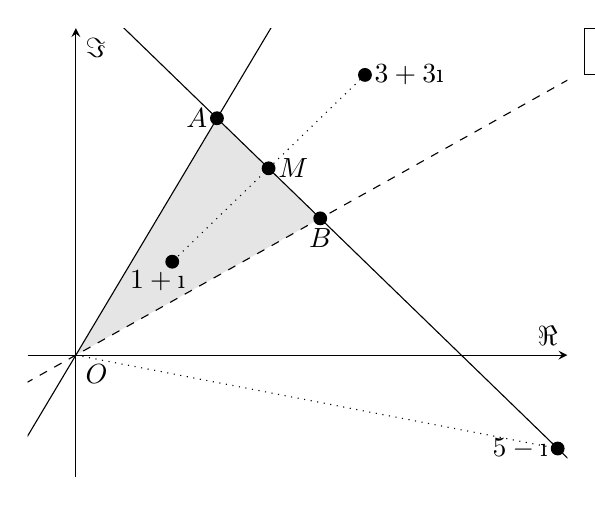
\begin{tikzpicture}[trim axis left, trim axis right]
                    \pgfdeclarelayer{pre main}
                    \pgfsetlayers{pre main,main}
                    \begin{axis}[
                        axis on top,
                        domain = -10:10 ,
                        samples = 101,
                        axis y line=middle,
                        axis x line=middle,
                        xtick = \empty,
                        ytick = \empty,
                        xmax=6/1.25 + 0.3,
                        xmin=-1/1.25 + 0.3,
                        ymin=-2/1.25 + 0.3,
                        ymax=4/1.25 + 0.3,
                        xlabel = {$\Re$},
                        ylabel = {$\Im$},
                        legend cell align={left},
                        legend pos=outer north east,
                        after end axis/.code={
                            \path (axis cs:0,0) 
                                node [anchor=north west] {$O$};
                            }
                        ]
                        \addlegendimage{line legend, black!10, line width=5pt}
                        \addlegendentry{required locus};
                        
                        \addplot[black] {-x + 4};
                        \addplot[black] {1.73 * x};
                        \addplot[dashed] {0.577 * x};

                        \coordinate (O) at (0, 0);
                        \coordinate[label=left:$A$] (A) at (1.464, 2.536);
                        \coordinate[label=below:$B$] (B) at (2.536, 1.464);

                        \pgfonlayer{pre main}
                            \fill[black!10] (0, 0) -- (A) -- (B) -- cycle;
                        \endpgfonlayer

                        \coordinate[label=right:$3 + 3\i$] (Z1) at (3, 3);
                        \coordinate (Z2) at (1, 1);
                        \draw[dotted] (Z1) -- (Z2);

                        \node at (0.85, 0.8) {$1 + \i$};

                        \fill (A) circle[radius=2.5pt];
                        \fill (B) circle[radius=2.5pt];
                        \fill (Z1) circle[radius=2.5pt];
                        \fill (Z2) circle[radius=2.5pt];

                        \coordinate[label=left:$5 - \i$] (Z3) at (5, -1);
                        \fill (Z3) circle[radius=2.5pt];
                        
                        \draw[dotted] (O) -- (Z3);

                        \coordinate[label=right:$M$] (M) at (2, 2);
                        \fill (M) circle[radius=2.5pt];
                    \end{axis}
                \end{tikzpicture}
            \end{center}
    \end{ppart}
    \begin{ppart}
        Note that the locus of $\abs{z - 3 - 3\i} = \abs{z - 1 - \i}$ has Cartesian equation $y = -x + 4$, while the loci of $\frac\pi6 = \arg{z}$ and $\arg{z} = \frac\pi3$ have Cartesian equations $y = \frac1{\sqrt3} x$ and $y = \sqrt3 x$ respectively. Let $A$ and $B$ be the intersections between $y = -x + 4$ with $y = \sqrt3 x$ and $y = \frac1{\sqrt3}x$ respectively.

        At $A$, we have $y = \sqrt3 x = -x + 4$, whence $A\bp{\frac4{1 + \sqrt3}, \frac{4\sqrt3}{1 + \sqrt3}}$. Thus, \[OA = \sqrt{\bp{\frac{4}{1 + \sqrt3}}^2 + \bp{\frac{4\sqrt3}{1 + \sqrt3}}^2} = \frac{8}{1 + \sqrt3}.\] By symmetry, we also have $OA = OB$. Finally, since $\angle AOB = \frac\pi3 - \frac\pi6 = \frac\pi6$, \[[\triangle AOB] = \frac12 (OA)(OB)\sin \angle AOB = \frac12 \bp{\frac8{1 + \sqrt3}}^2 \frac12 = \frac{16}{\bp{1 + \sqrt3}^2} = 4\bp{1 - \sqrt3}^2.\]
    \end{ppart}
    \begin{ppart}
        Observe that $\min \arg{z - (5 - \i)} = \frac34 \pi$ and $\max \arg{z - (5 -\i)} = \arctan \frac{-1}5 + \pi = \pi -\arctan \frac15 $. Hence, $\frac34 \pi \leq \arg{z - 5 + \i} < \pi-\arctan \frac15$.
    \end{ppart}
\end{solution}

\clearpage
\begin{problem}
    Sketch on an Argand diagram the set of points representing all complex numbers $z$ satisfying both inequalities
    \[
        \abs{\i z - 2\i - 2} \leq 2 \qquad \text{and} \qquad \Re{z} > \abs{1 + \sqrt3 \i}
    \]
    Find
    \begin{enumerate}
        \item the range of $\arg{z - 2 - 2\i}$,
        \item the complex number $z$ where $\arg{z - 2 - 2\i}$ is a maximum.
    \end{enumerate}

    The locus of the complex number $w$ is defined by $\abs{w - 5 + 2\i} = k$, where $k$ is a real and positive constant. Find the range of values of $k$ such that the loci of $w$ and $z$ will intersect.
\end{problem}
\begin{solution}
    Note $\abs{\i z - 2i - 2} \leq 2 \implies \abs{\i (z - 2 + 2i)} \leq 2 \implies \abs{z - (2 - 2\i)} \leq 2$ and $\Re{z} > \abs{1 + \sqrt3 \i} = 2$. 
    
    \begin{center}\tikzsetnextfilename{97}
        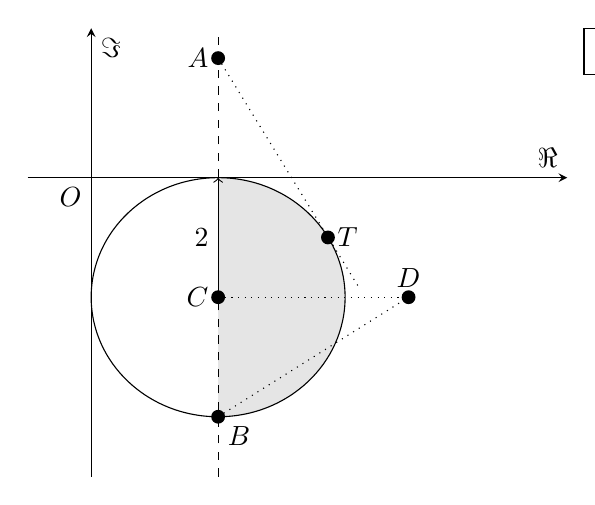
\begin{tikzpicture}[trim axis left, trim axis right]
            \pgfdeclarelayer{pre main}
            \pgfsetlayers{pre main,main}
            \begin{axis}[
                axis on top,
                domain = -10:10 ,
                samples = 101,
                axis y line=middle,
                axis x line=middle,
                xtick = \empty,
                ytick = \empty,
                xmax=7.5,
                xmin=-1,
                ymin=-5,
                ymax=2.5,
                xlabel = {$\Re$},
                ylabel = {$\Im$},
                legend cell align={left},
                legend pos=outer north east,
                after end axis/.code={
                    \path (axis cs:0,0) 
                        node [anchor=north east] {$O$};
                    }
                ]
                \addlegendimage{line legend, black!10, line width=5pt}
                \addlegendentry{required locus};

                \coordinate[label=left:$C$] (C) at (2, -2);
                \draw (C) circle[radius=2];
                \coordinate[label=above:$D$] (Z) at (5, -2);

                \fill (C) circle[radius=2.5pt];
                \fill (Z) circle[radius=2.5pt];

                \draw[dashed] (2, -5) -- (2, 2.5);

                \pgfonlayer{pre main}
                    \fill[black!10] (C) circle[radius=2];
                    \fill[white] (2, -4.5) rectangle (0, 0);
                \endpgfonlayer

                \draw[<->] (C) -- (2, 0);
                \node[anchor=east] at (2, -1) {2};

                \coordinate[label=below right:$B$] (B) at (2, -4);
                \draw[dotted] (C) -- (Z);
                \draw[dotted] (B) -- (Z);
                \fill (B) circle[radius=2.5pt];

                \coordinate[label=left:$A$] (A) at (2, 2);
                \fill (A) circle[radius=2.5pt];

                \addplot[dotted, domain=2:4.2] {-1.73 * (x-2) + 2};

                \fill (2 + 1.73, -1) circle[radius=2.5pt] node[anchor=west] {$T$};
            \end{axis}
        \end{tikzpicture}
    \end{center}

    \begin{ppart}
        Note $\abs{z - 2 - 2\i} = \arg{z - (2 + 2\i)}$. Let $A(2 + 2\i)$ and $C(2 - 2\i)$. Let $T$ be the point at which $AT$ is tangent to the circle. Then $\angle ATC = \frac\pi2$, $AC = 4$ and $TC = 2$. Hence, $\angle CAT = \arcsin \frac24 = \frac\pi6$. Thus, $\min \arg{z - 2 - 2\i} = -\frac\pi2$ and $\max \arg{z - 2 - 2\i} = \min \arg{z - 2 - 2\i} + \angle CAT = -\frac\pi2 + \frac\pi6 = -\frac\pi3$. Hence, $-\frac\pi2 < \arg{z - 2 - 2i} \leq -\frac\pi3$.
    \end{ppart}
    \begin{ppart}
        Relative to $C$, $T$ is given by $2 \bp{\cos \frac\pi6 + \i\sin \frac\pi6} = \sqrt3 + \i$. Thus, $T = (\sqrt 3 + \i) + (2 - 2\i) = 2 + \sqrt3 - \i$.
    \end{ppart}

    Note $\abs{w - 5 + 2\i} = k \implies \abs{w - (5 - 2\i)} = k$. Let $D(5 - 2\i)$. Observe that $CD$ is given by the sum of the radius of the circle and $\min k$. Hence, $\min k = 3 - 2 = 1$. Let $B(2 - 4\i)$. Then $\max k$ is given by the distance between $B$ and $D$. By the Pythagorean Theorem, we have $\max k = \sqrt{(5-2)^2 + (-2-(-4))^2} = \sqrt{13}$. Thus, $1 \leq k \leq \sqrt{13}$.
\end{solution}